\documentclass[11pt,a4paper]{article}

% --- Geometry & Typography ---------------------------------------------------
\usepackage[a4paper,top=2.0cm,bottom=2.0cm,left=2.2cm,right=2.2cm,footskip=1.0cm,headsep=0.4cm]{geometry}
\usepackage[T1]{fontenc}
\usepackage[utf8]{inputenc}
\usepackage{lmodern}
\usepackage{microtype}
\usepackage[dvipsnames,table]{xcolor}
\usepackage{titlesec}
\usepackage{enumitem}
\usepackage{booktabs}
\usepackage{array}
\usepackage{tabularx}
\usepackage{caption}
\usepackage{amsmath,amssymb}
\usepackage{tikz}
\usetikzlibrary{positioning,arrows.meta,shapes.geometric,fit,backgrounds,calc,decorations.pathreplacing,decorations.pathmorphing}
\usepackage{pgfgantt}
\usepackage{float}
\usepackage{multicol}

% --- Color palette (extracted from pitching deck + WSO2 PDF) -----------------
\definecolor{neuroblue}{HTML}{1F2D7A}
\definecolor{accentpurple}{HTML}{5E2D91}
\definecolor{swrorange}{HTML}{D55E00}
\definecolor{nodepeach}{HTML}{FAD7C7}
\definecolor{nodeblue}{HTML}{CFE2F3}
\definecolor{nodegreen}{HTML}{D9EAD3}
\definecolor{rulegrey}{HTML}{8A8A8A}
\definecolor{nodelilac}{HTML}{E0CFE8}

% --- Bibliography (natbib + custom apalike-comma style) --------------------
\usepackage[round,authoryear,sort&compress]{natbib}
\bibliographystyle{apalike}
\setcitestyle{aysep={,}}

% --- Section title styling ---------------------------------------------------
\titleformat{\section}
  {\color{neuroblue}\sffamily\large\bfseries}{\thesection.}{0.5em}{}[\vspace{-0.3em}\textcolor{accentpurple}{\rule{\linewidth}{0.4pt}}]
\titleformat{\subsection}
  {\color{neuroblue}\sffamily\normalsize\bfseries}{\thesubsection}{0.5em}{}
\titlespacing*{\section}{0pt}{0.45em}{0.15em}
\titlespacing*{\subsection}{0pt}{0.25em}{0.05em}

% --- Spacing tweaks ----------------------------------------------------------
\setlength{\parskip}{0.15em}
\setlength{\parindent}{0pt}
\renewcommand{\arraystretch}{1.0}
\captionsetup{font=small,labelfont={bf,color=neuroblue},skip=2pt}

% --- Hyperref (load last) ----------------------------------------------------
\usepackage[hidelinks]{hyperref}
\hypersetup{
  colorlinks=true,linkcolor=neuroblue,citecolor=neuroblue,urlcolor=neuroblue,
  pdftitle={HippoCortex Research Proposal},
  pdfauthor={Group 07, University of Kelaniya}
}

% --- Custom commands ---------------------------------------------------------
\newcommand{\objbold}[1]{\textbf{\color{neuroblue}#1}}

\begin{document}
\pagestyle{plain}

% =============================================================================
% TITLE BAND (compact, not full-page)
% =============================================================================
\begin{center}
{\sffamily\LARGE\bfseries HippoCortex}\\[0.2em]
{\itshape\small Biologically-Inspired Continual Learning via Sharp Wave Ripple Generative Replay in State Space Models}\\[0.7em]
{\footnotesize
\setlength{\tabcolsep}{4pt}\renewcommand{\arraystretch}{1.0}
\begin{tabular*}{0.82\linewidth}{@{\extracolsep{\fill}}ll@{}}
Hasinthaka Piyumal~~{\small(SE/2021/036)} & Praveen Dedigama~~{\small(SE/2021/031)} \\
Induwara Mihisara~~{\small(SE/2021/025)}  & Thagya Kavindi~~{\small(SE/2021/062)} \\
\end{tabular*}
}\\[0.45em]
{\itshape\footnotesize Group 07 \enspace\textbar\enspace Supervised by Dr.~Nalin Warnajith}
\end{center}

% =============================================================================
% 1. INTRODUCTION
% =============================================================================
\section{Introduction}

\subsection{Background}
Continual learning is the problem of training a neural network on a stream of tasks that arrive one after another, without losing what the network has already learned~\citep{delange2022continual}. Standard networks fail at this: as soon as a new task starts, the optimiser overwrites the weights that mattered for older tasks, and accuracy on those tasks collapses. The field calls this failure \emph{catastrophic forgetting}~\citep{kirkpatrick2017overcoming}. Three families of fixes exist (rehearsal, regularisation, and parameter isolation), but none of them works well for a robot that has to keep learning for months on a small on-board computer.

\subsection{Importance}
A robot that ships with a frozen model cannot pick up new terrain, new objects, or new operators once it leaves the factory. Sending its data to a cloud server for re-training drains battery, leaks private camera footage, and is unavailable offline. A learning rule that runs locally and uses a small, predictable memory budget per task would unlock genuine lifelong adaptation for the next generation of personal and service robots.

\subsection{Motivation}
The mammalian brain has already solved this problem. The hippocampus quickly stores fresh experience while the animal is awake, and during sleep it fires brief high-frequency bursts called \emph{sharp wave ripples} (SWRs). These bursts send \textbf{compressed} memory traces, not raw sensory recordings, to the neocortex for slow consolidation~\citep{buzsaki2015hippocampal,mcclelland1995complementary}. HippoCortex turns that idea into a trainable system. A State Space Model (SSM) backbone~\citep{gu2023mamba} replaces the usual replay buffer with a small generator that recreates plausible past activations on demand from a tiny summary of each old task.

% =============================================================================
% 2. PROBLEM STATEMENT
% =============================================================================
\section{Problem Statement}

The three existing families of continual-learning methods each break down for a deployed robot. \textbf{Rehearsal-based} methods such as iCaRL~\citep{rebuffi2017icarl} and Deep Generative Replay~\citep{shin2017continual} keep past data around or train a generator that produces full-resolution past inputs; both options grow with experience and raise privacy concerns. \textbf{Regularisation-based} methods such as EWC~\citep{kirkpatrick2017overcoming} add a penalty term that discourages important weights from changing, but tuning the penalty is fragile: too strong and the model stops learning, too weak and it forgets anyway. \textbf{Projection-based} methods, including GPM~\citep{saha2021gradient} and the recent SSM variants Mamba-CL~\citep{cheng2024mambacl} and Inf-SSM~\citep{lee2025exemplarfree}, instead constrain updates to a "safe" set of directions that should not disturb old weights; they are memory-efficient but their accuracy drops once the task stream passes about twenty tasks.

\textbf{No published method delivers all three of the following at once:} (i)~no raw data is ever stored; (ii)~the cost per training step is linear, so the method runs on an on-board edge processor; and (iii)~accuracy stays competitive on long task streams. HippoCortex targets exactly this gap. It replays \emph{synthetic hidden states} sampled from a per-task statistics buffer, then filters every gradient through a null-space projector, all on top of a Mamba SSM backbone.

\subsection{Research questions}
The work is organised around four research questions.
\textbf{RQ1:} can a per-task $(\mu,\sigma^{2})$ summary of internal features replace a raw-input replay buffer without sacrificing accuracy on long task streams?
\textbf{RQ2:} does a CVAE conditioned on task ID generate hidden states close enough to the true past distribution that a downstream classifier transfers within two percentage points?
\textbf{RQ3:} does combining null-space gradient projection with generative replay reduce forgetting more than either mechanism alone over twenty or more sequential tasks?
\textbf{RQ4:} does the integrated model fit the compute and memory budget of the Go2 Edu's on-board Jetson Orin NX at sub-50\,ms per-frame inference under a real-world task curriculum?

% =============================================================================
% 3. OBJECTIVES
% =============================================================================
\section{Objectives}

\begin{enumerate}[label=\textbf{O\arabic*.},leftmargin=2.2em,itemsep=0.05em,topsep=0.1em]
  \item \objbold{Compact statistics buffer.} A per-task memory that keeps only the mean $\mu$ and variance $\sigma^{2}$ of the backbone's features at one layer; size constant in the number of samples per task.
  \item \objbold{SWR generator.} A small Conditional VAE~\citep{sohn2015learning} that, given a task ID, samples past hidden states from the buffer; classifier transfer within two percentage points of real states.
  \item \objbold{Null-space gradient projector.} A step $P=I-UU^{\top}$ that strips each new-task gradient of components along directions important to earlier tasks; old-task accuracy drops $<\!3$ percentage points after twenty Split-CIFAR100 tasks.
  \item \objbold{Validation on standard benchmarks.} Evaluate on Split-CIFAR100 (20 $\times$ 5-class tasks) and ImageNet-R; target 8--10\% accuracy gain over Mamba-CL and $\sim$4\% over Inf-SSM.
  \item \objbold{Embodied extension.} Extend to a hybrid Mamba+Transformer~\citep{vaswani2017attention} stack on the Unitree Go2 Edu, with on-device Jetson Orin NX inference under 50\,ms per frame.
  \item \objbold{Publication.} Two peer-reviewed papers: Stage~1 algorithm and Stage~2 embodied deployment.
\end{enumerate}

% =============================================================================
% 4. PRELIMINARY LITERATURE REVIEW
% =============================================================================
\section{Preliminary Literature Review}

\subsection{Catastrophic forgetting}
\citet{kirkpatrick2017overcoming} introduced the modern fix, Elastic Weight Consolidation, which adds the penalty $\mathcal{L}_{\text{EWC}} = \mathcal{L}_{B} + \tfrac{\lambda}{2}\sum_{i} F_{i}(\theta_{i}-\theta_{i}^{*})^{2}$, where $F_i$ tells the optimiser how sensitive the past-task loss is to each weight. The penalty works for short streams but becomes brittle as tasks accumulate~\citep{delange2022continual}.

\subsection{Rehearsal and generative replay}
iCaRL~\citep{rebuffi2017icarl} keeps a fixed-size buffer of real past examples, so its storage grows with the number of classes seen. Deep Generative Replay~\citep{shin2017continual} avoids that by training a generator that synthesises raw past inputs, but training an image generator on the fly on an edge device is not realistic. HippoCortex replays in compressed hidden-state space instead of pixel space, which keeps the generator small enough to train on-device.

\subsection{Projection-based protection}
GPM~\citep{saha2021gradient} keeps a small set of basis vectors describing the directions in feature space that past tasks rely on, and projects new gradients onto the part of space orthogonal to that set. Mamba-CL~\citep{cheng2024mambacl} adapts the idea to selective SSMs, and Inf-SSM~\citep{lee2025exemplarfree} extends it using Grassmannian distances over an extended-observability subspace. Both keep the buffer empty, but accuracy still decays as the stream grows long. HippoCortex addresses that decay by adding a generative replay signal on top of the projection step.

\subsection{State space models for continual learning}
Mamba~\citep{gu2023mamba} introduces input-dependent state updates and approaches Transformer accuracy on a wide range of sequence tasks while running in linear time with constant memory per token. That is exactly what an on-device continual learner needs: long context without the quadratic cost of attention, and a clean internal structure in which the directions important to old tasks are easy to identify and protect.

\subsection{Biological grounding}
\citet{buzsaki2015hippocampal} reviews two decades of evidence that hippocampal SWRs (140--200~Hz bursts during sleep and immobility) replay waking neuronal sequences at roughly 10--20$\times$ time-compression and consolidate them into the neocortex. \citet{mcclelland1995complementary} formalises this as the \emph{complementary learning systems} hypothesis: the fast hippocampus and the slow neocortex avoid interference precisely because they exchange compressed traces rather than raw experience. HippoCortex inherits the same division of labour (Figure~\ref{fig:biomap}).

\subsection{Research gap}
Across the five strands above, no published method offers exemplar-free continual learning that stays stable on long task streams, runs on a linear-time backbone, and has been validated on a physical robot. Figure~\ref{fig:methodtable} lays out the gap HippoCortex fills.

% --- FIGURE 1: Bio mapping ---------------------------------------------------
\begin{figure}[ht]
\centering
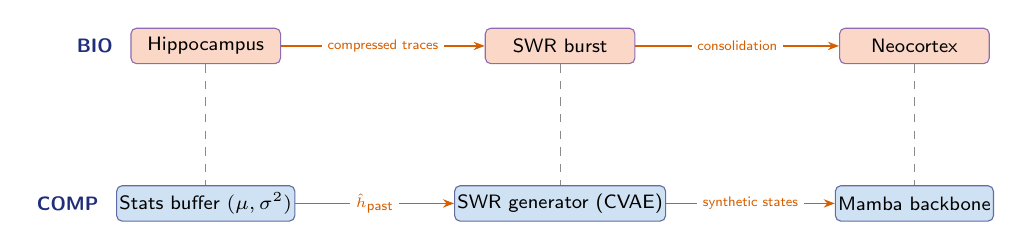
\begin{tikzpicture}[
  font=\sffamily\scriptsize,
  bionode/.style={rectangle,rounded corners=2pt,draw=accentpurple!70,fill=nodepeach,minimum width=1.9cm,minimum height=0.45cm,inner sep=1pt},
  cmpnode/.style={rectangle,rounded corners=2pt,draw=neuroblue!70,fill=nodeblue,minimum width=1.9cm,minimum height=0.45cm,inner sep=1pt},
  arr/.style={-{Stealth[length=4pt]},semithick,swrorange},
  dashlink/.style={dashed,thin,rulegrey},
  lanelabel/.style={font=\sffamily\scriptsize\bfseries,text=neuroblue},
  arrlabel/.style={font=\sffamily\tiny,text=swrorange,fill=white,inner xsep=2pt,inner ysep=0.5pt},
]
% Bio lane (top)
\node[bionode] (hipp)   at (0.5,1.5)  {Hippocampus};
\node[bionode] (swr)    at (5.0,1.5)  {SWR burst};
\node[bionode] (cortex) at (9.5,1.5)  {Neocortex};
\node[lanelabel,anchor=east] at ($(hipp.west)+(-0.1,0)$) {BIO};
\draw[arr] (hipp) -- node[arrlabel]{compressed traces} (swr);
\draw[arr] (swr)  -- node[arrlabel]{consolidation} (cortex);

% Computational lane (bottom)
\node[cmpnode] (sb)    at (0.5,-0.5) {Stats buffer $(\mu,\sigma^{2})$};
\node[cmpnode] (gen)   at (5.0,-0.5) {SWR generator (CVAE)};
\node[cmpnode] (mamba) at (9.5,-0.5) {Mamba backbone};
\node[lanelabel,anchor=east] at ($(sb.west)+(-0.1,0)$) {COMP};
\draw[arr] (sb)  -- node[arrlabel]{$\hat{h}_{\text{past}}$} (gen);
\draw[arr] (gen) -- node[arrlabel]{synthetic states} (mamba);

% Vertical analogy links
\draw[dashlink] (hipp)   -- (sb);
\draw[dashlink] (swr)    -- (gen);
\draw[dashlink] (cortex) -- (mamba);
\end{tikzpicture}
\caption{Mapping of biological consolidation onto HippoCortex components.}
\label{fig:biomap}
\end{figure}

% --- FIGURE 2: Method comparison table-as-figure -----------------------------
\begin{figure}[ht]
\centering
\footnotesize
\setlength{\tabcolsep}{4pt}
\begin{tabular*}{\linewidth}{@{\extracolsep{\fill}}lcccc@{}}
\toprule
\textbf{Method} & \textbf{Replay type} & \textbf{Raw data?} & \textbf{Memory cost} & \textbf{On robot?} \\
\midrule
EWC~\citep{kirkpatrick2017overcoming}              & none                    & no            & low (Fisher only)   & no \\
iCaRL~\citep{rebuffi2017icarl}                     & exemplar                & \textbf{yes}  & grows w/ classes    & no \\
DGR~\citep{shin2017continual}                      & raw-pixel generative    & no            & generator weights   & no \\
GPM~\citep{saha2021gradient}                       & null-space projection   & no            & basis matrices      & no \\
Mamba-CL~\citep{cheng2024mambacl}                  & null-space (SSM)        & no            & basis matrices      & no \\
Inf-SSM~\citep{lee2025exemplarfree}                & extended observability  & no            & subspace summaries  & no \\
\rowcolor{nodegreen}\textbf{\color{neuroblue}HippoCortex (ours)}  & \textbf{\color{neuroblue}SWR latent + null-space} & \textbf{\color{neuroblue}no} & \textbf{\color{neuroblue}compact summary per task} & \textbf{\color{neuroblue}yes (Go2)} \\
\bottomrule
\end{tabular*}
\caption{Comparison of continual-learning methods. HippoCortex is the only entry that combines latent generative replay with null-space protection on a linear-time SSM backbone, with planned validation on a physical robot.}
\label{fig:methodtable}
\end{figure}

% =============================================================================
% 5. METHODOLOGY
% =============================================================================
\section{Methodology}

The project runs in two stages. \textbf{Stage 1} (Months 1--3) builds the core algorithm and validates it on standard image benchmarks. \textbf{Stage 2} (Months 4--6) extends the model to a hybrid architecture and deploys it on the Unitree Go2 Edu quadruped. Hardware access for Stage 2 is already in hand: the team's separate hardware proposal to the WSO2 Call for Proposals on Unitree Go2 Edu Robot-based Projects has been \emph{approved}, which gives us access to the robot at the WSO2 Colombo office along with a project grant.

\subsection{Stage 1: Core algorithm (Months 1--3)}
HippoCortex chains four components, shown in Figure~\ref{fig:pipeline}:
\begin{itemize}[leftmargin=1.4em,itemsep=0.05em,topsep=0.1em]
  \item \textbf{Mamba backbone.} A selective SSM~\citep{gu2023mamba} that turns each input into a hidden-state vector.
  \item \textbf{Statistics buffer.} For every class we have seen, we store only the mean $\mu$ and variance $\sigma^{2}$ of the backbone's hidden states. Raw inputs are never kept.
  \item \textbf{SWR generator.} A Conditional VAE~\citep{sohn2015learning} that, given a task identifier, samples synthetic past hidden states $\hat{h}_{\text{past}}$ from the buffer.
  \item \textbf{Null-space projector.} We filter every gradient through $P=I-UU^{\top}$. The columns of $U$ list the directions in feature space that earlier tasks rely on~\citep{saha2021gradient,cheng2024mambacl}, so $P$ removes any update that would disturb them.
\end{itemize}

\textbf{Training loop (per new task).} For each new task we run three short passes. (i)~A \emph{warm-up} pass trains on the new task alone, without replay, so the backbone gets a sensible starting point. (ii)~A \emph{joint pass} mixes new-task features with synthetic $\hat{h}_{\text{past}}$ from the SWR generator, and routes every gradient through the projector before it touches a weight. (iii)~A \emph{consolidation} pass updates the statistics buffer with the new task and adds the new task's important directions to $U$.

\textbf{Benchmarks, baselines, metrics.}

\begin{center}\small
\begin{tabular}{@{}l p{0.74\linewidth}@{}}
\toprule
\textbf{Datasets}   & Split-CIFAR100 (20 tasks $\times$ 5 classes); ImageNet-R (rendition shift). \\
\textbf{Baselines}  & Naive fine-tuning, EWC~\citep{kirkpatrick2017overcoming}, DGR~\citep{shin2017continual}, Mamba-CL~\citep{cheng2024mambacl}, Inf-SSM~\citep{lee2025exemplarfree}. \\
\textbf{Metrics}    & Average accuracy, forgetting rate, memory footprint (MB) vs.\ task index. \\
\bottomrule
\end{tabular}
\end{center}

% --- FIGURE 3: Stage 1 pipeline ---------------------------------------------
\begin{figure}[ht]
\centering
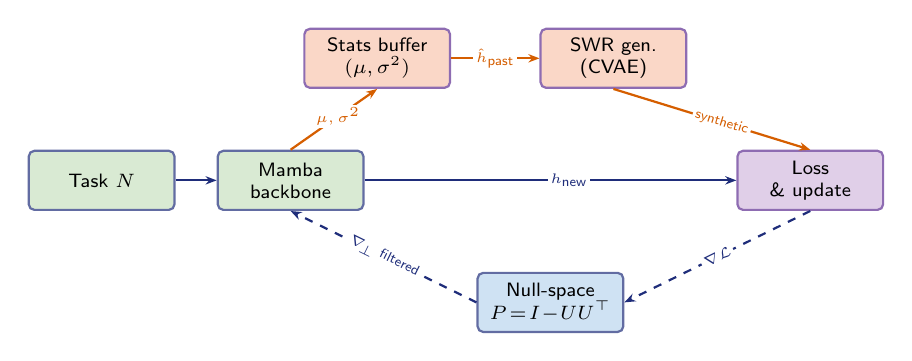
\begin{tikzpicture}[
  font=\sffamily\scriptsize,
  block/.style={rectangle,rounded corners=2pt,draw,thick,minimum height=0.75cm,minimum width=1.85cm,align=center,inner sep=2pt},
  inn/.style={block,fill=nodegreen,draw=neuroblue!70},
  buf/.style={block,fill=nodepeach,draw=accentpurple!70},
  proj/.style={block,fill=nodeblue,draw=neuroblue!70},
  term/.style={block,fill=nodelilac,draw=accentpurple!70},
  arr/.style={-{Stealth[length=4pt]},thick,neuroblue},
  swr/.style={-{Stealth[length=4pt]},thick,swrorange},
  fwdlbl/.style={font=\sffamily\tiny,text=neuroblue,fill=white,inner sep=1pt},
  swrlbl/.style={font=\sffamily\tiny,text=swrorange,fill=white,inner sep=1pt},
  graddlbl/.style={font=\sffamily\tiny,text=neuroblue,fill=white,inner sep=1pt},
]
% Top row: replay path
\node[buf] (sb)    at (3.5, 1.55) {Stats buffer\\$(\mu,\sigma^{2})$};
\node[buf] (gen)   at (6.5, 1.55) {SWR gen.\\(CVAE)};
% Middle row: forward path
\node[inn] (input) at (0,    0)   {Task $N$};
\node[inn] (mamba) at (2.4,  0)   {Mamba\\backbone};
\node[term] (loss) at (9.0,  0)   {Loss\\\& update};
% Bottom row: projection
\node[proj] (proj) at (5.7, -1.55){Null-space\\$P\!=\!I\!-\!UU^{\top}$};

% Forward pass (blue, solid)
\draw[arr] (input) -- (mamba);
\draw[arr] (mamba.east) -- node[fwdlbl,pos=0.55]{$h_{\text{new}}$} (loss.west);

% Replay path (orange, solid) -- straight diagonals, labels in open space
\draw[swr] (mamba.north) -- node[swrlbl,pos=0.55]{$\mu,\sigma^{2}$} (sb.south);
\draw[swr] (sb.east) -- node[swrlbl]{$\hat{h}_{\text{past}}$} (gen.west);
\draw[swr] (gen.south) -- node[swrlbl,sloped,pos=0.55]{synthetic} (loss.north);

% Gradient projection (dashed, blue) -- diagonals
\draw[arr,dashed] (loss.south) -- node[graddlbl,sloped,pos=0.5]{$\nabla\mathcal{L}$} (proj.east);
\draw[arr,dashed] (proj.west) -- node[graddlbl,sloped,pos=0.5]{$\nabla_{\!\perp}$ filtered} (mamba.south);
\end{tikzpicture}
\caption{Stage 1 HippoCortex pipeline: synthetic past hidden states from the SWR generator are mixed with new-task features; every parameter update is filtered by the null-space projector before reaching the Mamba backbone.}
\label{fig:pipeline}
\end{figure}

\subsection{Stage 2: Embodied deployment (Months 4--6)}
A pure Mamba stack underuses spatial structure in camera frames, so for the robot we move to a hybrid stack: \texttt{Sensor stream $\to$ Mamba $\to$ Transformer attention~\citep{vaswani2017attention} $\to$ Mamba $\to$ Output}. Mamba layers track temporal state efficiently; the Transformer attention layer pulls richer spatial features from the RGB camera and depth frames. The HippoCortex SWR module wraps the whole stack, so continual learning applies uniformly with no architectural changes. Inference runs on the Go2 Edu's Jetson Orin NX 16\,GB (100 TOPS). The robot will work through a four-task curriculum: terrain recognition, object interaction, human-proximity awareness, and new-environment mapping. Implementation uses Python~3.11, PyTorch~2.x, ROS2, and Mujoco / Isaac~Sim for pre-deployment validation.

% =============================================================================
% 6. EXPECTED PROJECT DELIVERABLES
% =============================================================================
\section{Expected Project Deliverables}

\begin{itemize}[leftmargin=1.4em,itemsep=0.0em,topsep=0.05em]
  \item \objbold{Open-source reference implementation} (PyTorch, GitHub) of the full HippoCortex stack with reproducible training scripts and pre-trained checkpoints.
  \item \objbold{Stage 1 benchmark report} on Split-CIFAR100 and ImageNet-R: average accuracy, forgetting rate, memory footprint, and full per-component ablations against EWC, DGR, Mamba-CL and Inf-SSM.
  \item \objbold{Stage 1 paper} (peer-reviewed) describing the core algorithm and Stage 1 results.
  \item \objbold{Hybrid Mamba + Transformer extension} that wraps the SWR module around the hybrid stack for richer visual input.
  \item \objbold{Embodied demonstration} on the Go2 Edu running the four-task curriculum (terrain, object interaction, human proximity, environment mapping) on-device, with logged latency and per-task accuracy.
  \item \objbold{Stage 2 paper and thesis chapter} documenting the full embodied evaluation.
\end{itemize}

% =============================================================================
% 7. PROJECT SCHEDULE
% =============================================================================
\section{Project Schedule}

% --- FIGURE 5: Gantt (Apr 2026 -- Sep 2026, twelve half-month columns) -----
\begin{figure}[!ht]
\centering
\begin{ganttchart}[
  hgrid={*1{draw=gray!30,thin}},
  vgrid={*1{draw=gray!30,very thin}},
  x unit=0.78cm,
  y unit chart=0.42cm,
  y unit title=0.5cm,
  bar height=0.62,
  bar top shift=0.18,
  bar/.append style={draw=neuroblue!80,fill=neuroblue!35,rounded corners=1.5pt},
  bar label font=\sffamily\scriptsize,
  bar label node/.append style={align=right,text width=5.5cm},
  group/.append style={draw=accentpurple,fill=accentpurple!55,rounded corners=1.5pt},
  group label font=\sffamily\scriptsize\bfseries,
  group label node/.append style={text=accentpurple},
  group peaks width=0,
  group peaks height=0,
  group left shift=0,
  group right shift=0,
  group top shift=0.15,
  group height=0.7,
  milestone/.append style={fill=swrorange,draw=swrorange!70!black},
  milestone label font=\sffamily\tiny\bfseries,
  milestone label node/.append style={text=swrorange!70!black},
  milestone height=0.5,
  milestone top shift=0.25,
  title label font=\sffamily\scriptsize\bfseries,
  title/.append style={draw=accentpurple!70,fill=accentpurple!10},
  title height=1,
  ]{1}{12}
  \gantttitle{Apr 2026}{2} \gantttitle{May}{2} \gantttitle{Jun}{2} \gantttitle{Jul}{2} \gantttitle{Aug}{2} \gantttitle{Sep 2026}{2} \\
  \ganttgroup{Stage 1: Core algorithm}{1}{6} \\
  \ganttbar{T1 Literature review \& knowledge base}{1}{2} \\
  \ganttbar{T2 Proposal development \& submission}{1}{2} \\
  \ganttbar{T3 Stage 1 core: Mamba + projector}{2}{3} \\
  \ganttbar{T4 Stage 1 replay: stats buffer + SWR generator}{3}{4} \\
  \ganttbar{T5 Stage 1 benchmarking \& ablations}{4}{5} \\
  \ganttbar{T6 Stage 1 paper draft \& submission}{5}{6} \ganttmilestone[inline=false]{}{6} \\
  \ganttgroup{Stage 2: Embodied deployment}{6}{12} \\
  \ganttbar{T7 Hybrid Mamba + Transformer}{6}{7} \\
  \ganttbar{T8 Simulator integration \& curriculum}{7}{9} \\
  \ganttbar{T9 Robot deployment on Go2 Edu}{8}{11} \\
  \ganttbar{T10 Real-world experiments}{11}{11} \\
  \ganttbar{T11 Stage 2 paper \& thesis}{10}{12} \ganttmilestone[inline=false]{}{12}
\end{ganttchart}\\[0.2em]
\hspace*{6.0cm}\textcolor{swrorange!70!black}{\sffamily\tiny\bfseries$\blacklozenge$~Paper 1 (mid Jun)\quad$\blacklozenge$~Paper 2 + release (mid Sep)}
\caption{Six-month project schedule (April--September 2026). Each column is a half-month. Stage 1 delivers the core algorithm and first paper by late June; Stage 2 covers the hybrid extension, simulator validation, on-device robot deployment, real-world experiments, and the final paper / thesis.}
\label{fig:gantt}
\end{figure}

\subsection{Team responsibilities}
The Gantt above lists each task's lead. Per-member ownership is summarised below.

\begin{center}\small
\begin{tabularx}{\linewidth}{@{}l l X@{}}
\toprule
\textbf{Member} & \textbf{ID} & \textbf{Primary responsibility} \\
\midrule
Hasinthaka Piyumal & SE/2021/036 & Team lead, research direction, training pipeline, paper writing, WSO2 liaison. \\
Praveen Dedigama   & SE/2021/031 & Mamba backbone, null-space projector, hybrid stack design. \\
Induwara Mihisara  & SE/2021/025 & Biological grounding, data loaders, simulator integration. \\
Thagya Kavindi     & SE/2021/062 & Evaluation metrics, benchmark runs, ablation studies, results analysis. \\
\bottomrule
\end{tabularx}
\end{center}

% =============================================================================
% 7. REFERENCES
% =============================================================================
\section{References}
{\footnotesize
\setlength{\bibsep}{0.05em}
\renewcommand{\section}[2]{}% suppress duplicate heading produced by thebibliography
\begin{thebibliography}{12}
\bibitem[Buzs\'aki, 2015]{buzsaki2015hippocampal}
Buzs\'aki, G. (2015). Hippocampal sharp wave-ripple: A cognitive biomarker for episodic memory and planning. \emph{Hippocampus}, 25(10), 1073--1188.

\bibitem[Cheng et al., 2024]{cheng2024mambacl}
Cheng, D., Huang, Y., Zhang, J., Chen, K., Liu, M., \& Huang, Q. (2024). Mamba-CL: Optimizing selective state space model in null space for continual learning. \emph{arXiv preprint arXiv:2411.15469}.

\bibitem[De Lange et al., 2022]{delange2022continual}
De Lange, M., Aljundi, R., Masana, M., Parisot, S., Jia, X., Leonardis, A., Slabaugh, G., \& Tuytelaars, T. (2022). A continual learning survey: Defying forgetting in classification tasks. \emph{IEEE Transactions on Pattern Analysis and Machine Intelligence}, 44(7), 3366--3385.

\bibitem[Gu \& Dao, 2023]{gu2023mamba}
Gu, A., \& Dao, T. (2023). Mamba: Linear-time sequence modeling with selective state spaces. \emph{arXiv preprint arXiv:2312.00752}.

\bibitem[Kirkpatrick et al., 2017]{kirkpatrick2017overcoming}
Kirkpatrick, J., Pascanu, R., Rabinowitz, N., Veness, J., Desjardins, G., Rusu, A.~A., Milan, K., Quan, J., Ramalho, T., Grabska-Barwinska, A., Hassabis, D., Clopath, C., Kumaran, D., \& Hadsell, R. (2017). Overcoming catastrophic forgetting in neural networks. \emph{Proceedings of the National Academy of Sciences}, 114(13), 3521--3526.

\bibitem[Lee et al., 2025]{lee2025exemplarfree}
Lee, I.~N., Mahmoodi, L., Le, T., \& Harandi, M. (2025). Exemplar-free continual learning for state space models. \emph{arXiv preprint arXiv:2505.18604}.

\bibitem[McClelland et al., 1995]{mcclelland1995complementary}
McClelland, J.~L., McNaughton, B.~L., \& O'Reilly, R.~C. (1995). Why there are complementary learning systems in the hippocampus and neocortex: Insights from the successes and failures of connectionist models of learning and memory. \emph{Psychological Review}, 102(3), 419--457.

\bibitem[Rebuffi et al., 2017]{rebuffi2017icarl}
Rebuffi, S.-A., Kolesnikov, A., Sperl, G., \& Lampert, C.~H. (2017). iCaRL: Incremental classifier and representation learning. In \emph{Proceedings of the IEEE Conference on Computer Vision and Pattern Recognition (CVPR)} (pp.~2001--2010).

\bibitem[Saha et al., 2021]{saha2021gradient}
Saha, G., Garg, I., \& Roy, K. (2021). Gradient projection memory for continual learning. In \emph{International Conference on Learning Representations (ICLR)}.

\bibitem[Shin et al., 2017]{shin2017continual}
Shin, H., Lee, J.~K., Kim, J., \& Kim, J. (2017). Continual learning with deep generative replay. In \emph{Advances in Neural Information Processing Systems (NeurIPS)}.

\bibitem[Sohn et al., 2015]{sohn2015learning}
Sohn, K., Lee, H., \& Yan, X. (2015). Learning structured output representation using deep conditional generative models. In \emph{Advances in Neural Information Processing Systems (NeurIPS)}.

\bibitem[Vaswani et al., 2017]{vaswani2017attention}
Vaswani, A., Shazeer, N., Parmar, N., Uszkoreit, J., Jones, L., Gomez, A.~N., Kaiser, \L., \& Polosukhin, I. (2017). Attention is all you need. In \emph{Advances in Neural Information Processing Systems (NeurIPS)}.
\end{thebibliography}
}

\end{document}
